\documentclass[12pt,a4paper,Flow]{report}
\usepackage[left=2.8cm,right=2.8cm,top=2.5cm,bottom=2cm]{geometry}
\usepackage[BoldFont]{xeCJK}
\usepackage{xeCJK}
\usepackage{graphicx}
\usepackage{float}
\usepackage{indentfirst}
\usepackage{fancyhdr}
\usepackage[toc,header,title]{appendix}
\usepackage{color,xcolor}
\usepackage{listings}
\usepackage{tikz}
\defaultfontfeatures{Mapping=tex-text}
\definecolor{llgray}{rgb}{0.9,0.9,0.9}
\lstloadlanguages{python}
\lstset{
  language=python,tabsize=4,keepspaces=true,
  xleftmargin=2em,xrightmargin=2em,aboveskip=1em,
  frame=none,
  commentstyle=\color{red}\itshape, % blue comments
  keywordstyle=\color{blue}\bfseries,
  backgroundcolor=\color{llgray},
  breakindent=22pt,
  numbers=left,stepnumber=1,numberstyle=\tiny,
  basicstyle=\footnotesize,
  showspaces=false,
  showstringspaces=false, % show explicit string spaces
  flexiblecolumns=false,%true,
  breaklines=true,breakautoindent=true,breakindent=4em,
  escapeinside={/*@}{@*/}
}
\usepackage[a4paper,CJKbookmarks,bookmarks=true,bookmarksopen=true]{hyperref}%很强大的一个东西
\hypersetup{
  pdftitle={},
  pdfauthor={Wang Pei},
  pdfkeywords={},
  bookmarksnumbered,
  breaklinks=true,
  pdfview=FitV,       % Or try pdfstartview={FitV}, This lead to uncorre
  urlcolor=cyan,
  colorlinks=true,
  citecolor=magenta,          %citeref's color
  linkcolor=blue,
}
\usepackage{titlesec}
\titleformat{\chapter}{\centering\huge}{\textbf{第}\thechapter{} \textbf{章}}{1em}{\textbf}
\renewcommand\contentsname{目录}
\renewcommand{\appendixpagename}{附录}
\renewcommand{\appendixname}{附录}
\setmainfont{DejaVu Sans}
\setCJKmainfont[BoldFont=WenQuanYi Micro Hei]{SimSun}

\begin{document}
\title{\textbf{体系结构实习——UniCore2模拟器\\实习报告}}
\author{张番栋 00848180\\刘澜涛 00848200\\王 沛 00848205\\CS08}
\date{\today}
\maketitle
\tableofcontents
\newpage
\chapter{实习内容}
\section{目标}
实习的主要内容是用C语言编写一个支持UniCore2精简指令系统的模拟器,并对其进行测试、验证。在之后的报告中,均称实习所完成的模拟器为MinSim。MiniSim的首要目标是进行正确的功能模拟,在此基础上增加对CPU流水线以及Cache的结构模拟,另外还有对程序动态运行情况的统计。MiniSim采用五级流水结构,和真实的UniCore2处理器并不相同。模拟的Cache则具有较灵活的定制性。\\
\section{具体实现功能}
\indent MiniSim支持的UniCore2指令子集中包含五类指令:
\begin{itemize}
\item 数据处理指令
\item 乘法和乘加指令
\item 跳转切换指令
\item 单数据传输指令
\item 条件转移指令和带链接条件转移指令。
\end{itemize}
\indent 从中可以看出,MiniSim并未对处理器特权状态的相关功能进行模拟,进而无法完全支持基于现代操作系统下的大部分程序。针对这个问题,我们做了一些工作,使得MiniSim在接受标准ELF文件作为输入的情况下,仍然能够完成大部分应用级别的功能模拟。\\
\indent 本次实习是与编译实习联合进行,因此我们在完成实习的过程中做了一些编译器和模拟器之间的协调工作。\\
\indent 最后,为了方便使用和调试,我们为MiniSim编写了一个简单的控制台模块,使得MiniSim在运行时可以设置断点,单步执行、查看寄存器、内存和流水线的状态。
\chapter{模拟器的存储体系}
\section{寄存器堆}
MiniSim以UniCore2处理器为目标进行模拟,因此寄存器堆的结构基本与之相同。有所区别的是,由于MiniSim无法处理异常(Exception),也不区分处理器状态,所以不需要SMSR标志寄存器。因此MiniSim共有32个通用寄存器和一个CMSR标志寄存器。
\section{内存管理}
MiniSim在运行时需要在自己的地址空间内同时维护目标程序的地址空间,因此需要建立一套面向目标程序的虚拟内存机制。在这个问题上,MiniSim采用的是页式内存管理机制。对于目标程序的32位地址空间,MiniSim进行了如下划分
\begin{itemize}
\item 31-25 位: 一级页表偏移
\item 24-15 位: 二级页表偏移
\item 14-0 位: 页内偏移
\end{itemize}
\begin{figure}[H]
  \centering
  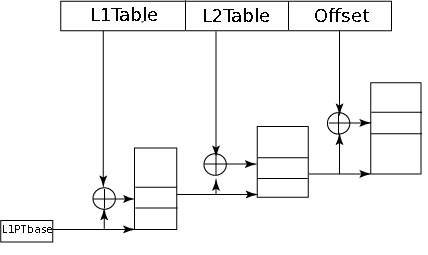
\includegraphics[width=0.5\textwidth]{pt.png}
\end{figure}
这样的结构表明页的大小为32KB。一级页表常驻内存,共有128个页表项,每个页表项大小为4B,即指向二级页表的指针。每个二级页表含有1024个页表项,每个页表项8B,存储的信息包括其所指向的页的起始地址和该页的读、写、执行属性。\\
\indent 这是一个很经典的虚拟内存管理机制,尤其在管理目标程序的栈时可以提供较好的局部性。在这种机制下,只要模拟器的存储管理模块要提供读、写内存的操作接口,真正执行目标程序的模块就可以减少很多工作量。同时,页式结构在一定程度上阻止非法的内存访问。
\section{Cahce}
MiniSim的Cache采取可定制结构,即用户可通过提供不同参数来获得不同的Cahce组织方式和Cache维护策略。我们共提供3种Cache更新策略(LRU,随机,轮转)和2种Cache写回策略(直写和回写)。
\chapter{模拟器运行环境的建立}
MiniSim接受标准ELF文件作为输入。在真正模拟运行目标机程序之前,需要做一些初始化工作。换言之,MiniSim需要完成一部分装载器和操作系统的工作。主要内容有ELF文件解析
内存环境的建立、代码段和数据段的载入、寄存器堆和流水线的初始化等等。
\section{对系统相关指令、功能的处理}
由于MiniSim不支持操作系统级别的指令,同时也不需要支持复杂的程序运行环境,所以模拟区间仅限于main函数。也就是说,MiniSim会跳过main函数之前的代码段,待main函数结束后退出。另外,为了便于检查,MiniSim还需要支持整型数据的非格式化输出。输出是与系统调用有关的功能,因此需要做一些约定:在给予MiniSim的输入中,输出功能要被封装在一个特定的函数中。当模拟进行到这个函数时,模拟器会以宿主机的输出调用替代之,然后结束该函数,从返回地址继续执行。为了达到这个目的,需要在ELF文件装载阶段进行一些工作。
\section{ELF文件解析}
需要做的工作主要有两点,具体的流程与ELF文件结构关系密切,这里只进行简单讨论。(ELF文件结构在elf.h头文件中定义。)
\subsection{关键函数的入口地址}
关键函数指的是main函数和输出封装函数。前者的入口是模拟程序的入口,后者的入口则决定了模拟器调用宿主输出机制的时机。大致流程如下:
\begin{enumerate}
\item 找到.shstrtab节区。
\item 遍历所有节区, 找到类型为 SHT\_SYMTAB 的两个节区:.symtab和.strtab。
\item 遍历.symtab节区, 找到需要的函数符号。
\item 返回其虚拟地址。
\end{enumerate}
\subsection{装载程序段}
获得ELF文件中代码段和数据段的位置和大小,以备建立模拟内存环境之用。
\begin{enumerate}
\item 获取程序段表 (Program Header Table) 基址
\item 遍历程序段表, 找到所有类型为 PT\_LOAD 的段。一般只有2个,分别存放代码、只读数据和可读写数据。
\item 根据段的大小和段需要的起始虚拟地址开辟新页,将段的数据从文件装入内存。
\end{enumerate}
\subsection{寄存器堆的初始化}
寄存器堆中有一些重要的寄存器需要在执行程序前进行必要的初始化。需要初始化的寄存器主要有4个:
\begin{enumerate}
\item PC。在运行程序前,需要在PC中装入之前解析ELF文件所得到的main函数入口地址。
\item LR。为了让MiniSim能够检测到main函数的结束,需要给LR一个特殊的值(一般是指向保留的地址空间,MiniSim在实现时采用了0这个特殊值)。这样当PC等于这个特殊值是,MiniSim就可以确定main函数已经结束,从而结束对目标程序的模拟执行。
\item SP。该寄存器的初始值决定了目标程序的栈的起始位置。在MiniSim的视线中,SP被初始化为0xf0000000。
\item FP。该寄存器的初始值决定了main函数栈帧的基址,因此需要给予与SP相同的初始值。
\end{enumerate}
\chapter{流水线设计}
\section{整体结构}
\subsection{设计描述}
MiniSim在完成指令功能模拟的同时,以软件的形式模拟了处理器的流水线结构。MiniSim的流水线分为取指(IF),译码(ID),执行(EX),访存(MEM),写回(WB)五级。由于软件不可能实现真正的并发,所以MiniSim的流水线实际上是以从WB到IF的顺序分步执行的。虽是如此,在真实流水线存在的与并发有关的问题在MiniSim中还是有所体现,比如数据和控制冒险。解决这些问题将是流水线设计和实现的重点。下图为流水线的基本结构:
\usetikzlibrary{positioning}
\usetikzlibrary{shadows}
\usetikzlibrary{shapes}
\begin{center}
\scalebox{1.1}
         {
  \begin{tikzpicture}[node distance=0.5cm]
    \node[fill=blue!20] (wb){WB};
    \node[fill=white] (wbin)[below =of wb]{数据传递};
    \node[fill=blue!20] (mem)[below =of wbin]{MEM};
    \node[fill=white] (memin)[below =of mem]{数据传递};
    \node[fill=blue!20] (ex)[below =of memin]{EX};
    \node[fill=white] (exin)[below =of ex]{数据传递};
    \node[fill=blue!20] (id)[below =of exin]{ID};
    \node[fill=blue!20] (ctrl)[right= of id]{控制};
    \node[fill=white] (idin)[below = of id]{数据传递};
    \node[fill=blue!20] (if)[below =of idin]{IF};
    \node[fill=red!40] (reg)[left= of wb]{寄存器堆};
    \node[fill=red!40,node distance=2cm] (memory)[right = of mem]{内存};
    \node[fill=red!40] (fwd) [left=of id]{前递单元};
    \draw[<->] (memory) -- (mem);
    \draw[<-] (fwd) -- (reg);
    \draw[->] (fwd) -- (id);
    \draw[->] (id) -- (ctrl);
    \draw[->] (ctrl) |- (exin);
    \draw[->] (wbin) -- (wb);
    \draw[->] (mem) -- (wbin);
    \draw[->] (memin) -- (mem);
    \draw[->] (ex) -- (memin);
    \draw[->] (exin) -- (ex);
    \draw[->] (id) -- (exin);
    \draw[->] (idin) -- (id);
    \draw[->] (if) -- (idin);
    \draw[<-] (if) -| (fwd);
    \draw[->] (ex) -- ++(-4,0) -- ++(0,-1) |-  (fwd);
    \draw[->] (mem) -- ++(-3.5,0) -- ++(0,-1) |- (fwd);
    \draw[->] (wb) -| (reg);
  \end{tikzpicture}
}
\end{center}
\subsection{程序实现}

\section{数据冒险相关}
由于数据冒险和控制冒险问题影响着整个流水线的运行,所以在描述各个流水级之前,先对MiiSim解决数据冒险的机制和策略做一介绍。
\subsection{两种数据冒险}
在MiniSim中,影响流水线运行的数据冒险实际上只有RAW一种。根据解决方式的不同,将之划分为两种:
\begin{enumerate}
\item 第一种RAW数据冒险是由数据处理指令产生的。在这种情况下,可以对数据处理指定的结果进行前递来满足后续指令的数据需求。
\item 第二种RAW数据貌相是由加载指令产生的。因为加载指令的结果在MEM阶段才会产生,所以无法通过前递满足紧随其后的一条指令的需求。如果此时发生数据相关,只能通过暂停流水线来解决。我们称这种情况为加载互锁。
\end{enumerate}
\subsection{数据冒险的解决}
\begin{enumerate}
\item 数据前递。数据前递的实现方法是在流水线状态信息(数据结构为PipeState)的ID\_input域中加入了三个前递数据槽。其中两个接受EX流水级前递的数据,一个接受MEM流水级前递的数据。为EX设立两个数据槽的原因是,UniCore2指令集中的访存指令对基址寄存器可以进行回写。因此相邻的两条指令中可能产生多达4次的回写。同时Unicore32指令最多可以有3个源寄存器。基于以上事实可知,仅仅两个数据槽不能满足所有的前递要求。因此需要为EX阶段增加一个数据槽。MEM阶段因为距离WB阶段只有1个周期,因此只需要有一个数据槽即可。
\item 加载互锁。加载互锁的实现比较简单,只需在ID阶段判断是否前一个流水级是否为load指令,该load指令与当前ID阶段的指令是否有数据相关即可。发生相关的条件是要读取的寄存器号与需要回写的寄存器号相同。由于流水线和模拟器流程执行顺序的关系,ID阶段要判断的回写信息存储在流水线状态中的mem\_in一级。当然,如果ID之后的流水级中插入了气泡,那么判断无需暂停流水线。
\end{enumerate}
\indent 因此对于数据冒险问题的解决可以概括如下:\\
\indent 在数据前递方面,前递的信息来自与回写信号,即wb\_dest\_sel。为EX设立的两个数据槽形成一个队列,第一个数据槽永远保存最新一次的前递信息。\\
\indent 读寄存器堆方面,首先判断是否需要进行加载互锁,如果是,暂停流水线,否则要扫描前递槽。需要注意的是EX数据前递槽的第二个槽要最后扫描,如果命中则取数据。未命中,则直接从寄存器堆取数据。
\section{取值(IF)阶段}
IF阶段完成的工作是取值,判断关键入口并进行处理,或者判断模拟是否已经结束。
\subsection{取指令}
IF阶段中会根据寄存器堆中PC的值访问存储器(借口由存储管理模块提供),并在取值结束后对PC进行更新(加4操作)。\\
\indent 值得注意的是,由于UniCore2指令系统中的PC对汇编程序是可见的,所以程序员可以将PC作为数据处理指令的目的寄存器使用。由于每一次PC的非累加性更改都相当与一次跳转,所以我们希望对与PC的修改可以尽早被探测到。因此,需要考虑PC的前递问题。\\
\indent 这也就是说,在取指令时不能依赖当前的PC值,而是需要先检查前递单元中是否有指向PC的前递。如果有,则要根据前递值去取指,并根据前递来源来清空流水线。如果前递来自EX阶段,则需要清空从ID到MEM的所有流水级。需要清空MEM的原因是,由于流水线倒序执行,到IF得到前递值时,制造前递的指令实际上已经从EX流水级进入了MEM。同理,如果前递来自较早的EX阶段或者MEM阶段,需要将从ID到WB的所有流水级排空。\\
\indent 可以看到,这样对PC的操作会对流水线产生非常不利的影响。因此我们约定在编译器中绝对不会通过直接修改PC来实现跳转。
\subsection{对关键函数入口地址的处理}
最初已经提到,我们的模拟器无法处理与处理器特权态有关的指令,加之编译器方面的限制,只能支持一种与系统调用有关的行为,即输出一个整数。在模拟器执行指令前的ELF文件载入工作中已经获得了封装输出子例程的函数入口。IF阶段要做的就是判断当前的PC是否为这个关键入口,如果是,则IF向ID送出一条伪指令,编码为0xffffffff。这条指令在ID阶段会被进行特殊处理。
\subsection{模拟结束的时机}
对结束模拟执行时机的判断也在IF阶段进行。同时将lr寄存器的值设置为0。这样一旦在IF阶段发现PC为全0,就可以认为模拟即将结束了。此时IF阶段会在产生4个汽泡后(带其他流水级中的指令执行完毕),产生结束模拟的信息。

\chapter{模拟器控制台}

\chapter{测试与验证}
\end{document}
